% To regenerate:
% cd vignettes/figures && pdflatex -interaction=nonstopmode -halt-on-error dag.tex && dvisvgm --pdf dag.pdf -o dag.svg && rm -f dag.aux dag.log dag.pdf
\documentclass[tikz,border=3pt]{standalone}
\usetikzlibrary{arrows.meta,positioning}

\begin{document}
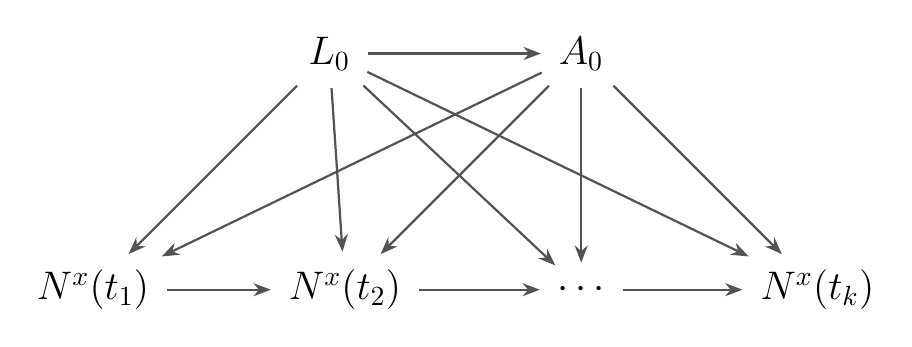
\begin{tikzpicture}[
  >={Stealth[length=2.2mm]},
  var/.style={font=\Large},
  every edge/.style={
    draw,
    ->,
    thick,
    gray!65!black,
    shorten >=3pt,
    shorten <=3pt
  }
]

  % Event history: the main visual axis
  \node[var] (N1) at (0,0)   {$N^x(t_1)$};
  \node[var] (N2) at (3.2,0) {$N^x(t_2)$};
  \node[var] (dots) at (6.2,0) {$\cdots$};
  \node[var] (Nk) at (9.2,0) {$N^x(t_k)$};

  % Baseline variables
  \node[var] (L0) at (3.0,3.0) {$L_0$};
  \node[var] (A0) at (6.2,3.0) {$A_0$};

  % Baseline treatment assignment
  \path (L0) edge (A0);

    % Baseline effects on event process
  \path (L0) edge (N1);
  \path (L0) edge (N2);
  \path (L0) edge (dots);
  \path (L0) edge (Nk);

  \path (A0) edge (N1);
  \path (A0) edge (N2);
  \path (A0) edge (dots);
  \path (A0) edge (Nk);

  % Event history feeding forward
  \path (N1) edge (N2);
  \path (N2) edge (dots);
  \path (dots) edge (Nk);

\end{tikzpicture}
\end{document}